\documentclass[twoside]{article}

\usepackage[math]{kurier}
\usepackage[sc]{mathpazo}                   
\renewcommand{\sfdefault}{kurier}
\usepackage{siunitx}
\usepackage{graphicx}
\usepackage{subfig}
\graphicspath{ {images/} }
% \usepackage{caption}
% \usepackage{subcaption}

\usepackage{amsmath}
\setlength{\oddsidemargin}{0.25 in}
\setlength{\evensidemargin}{-0.25 in}
\setlength{\topmargin}{-0.6 in}
\setlength{\textwidth}{6.5 in}
\setlength{\textheight}{8.5 in}
\setlength{\headsep}{0.75 in}
\setlength{\parindent}{0 in}
\setlength{\parskip}{0.1 in}


\newcounter{lecnum}
\renewcommand{\thepage}{\thelecnum-\arabic{page}}
\renewcommand{\thesection}{\thelecnum.\arabic{section}}
\renewcommand{\theequation}{\thelecnum.\arabic{equation}}
\renewcommand{\thefigure}{\thelecnum.\arabic{figure}}
\renewcommand{\thetable}{\thelecnum.\arabic{table}}


\newcommand{\lecture}[4]{
   \pagestyle{myheadings}
   \thispagestyle{plain}
   \newpage
   \setcounter{lecnum}{#1}
   \setcounter{page}{1}
   \noindent
   \begin{center}
   \framebox{
      \vbox{\vspace{2mm}
    \hbox to 6.28in { {\bf \sffamily AA 274: Principles of Robotic Autonomy
                        \hfill Winter 2018} }
       \vspace{4mm}
       \hbox to 6.28in { {\sffamily{\Large \hfill Lecture #1: #2  \hfill}} }
       \vspace{2mm}
       \hbox to 6.28in { {\it \hfill Scribes: #4} }
      \vspace{2mm}}
   }
   \end{center}
   \markboth{Lecture #1: #2}{Lecture #1: #2}

   \vspace*{4mm}
}



%%%%%%%%%%%%%%%%%%%%%%%%%%
%document
\begin{document}
%modify this
\lecture{8}{Information Extraction, Machine Learning for Robot Autonomy}{}{Richard Akira Heru, Tarun Punnoose, Dhruv Samant, Vince Chiu, Vincent Chow, Ayush Gupta}

\section{Introduction}
The goal of this lecture is to learn techniques for information extraction. Our particular focus in this lecture will be on: 1) Finding geometric primitives to assist in robot's localization and mapping; and 2) Object recognition and scene understanding that is useful for autonomous robots in ways such as localization within a topological map and for high-level reasoning.

However, sensor measurements are susceptible to noise. Therefore, we first need to discuss the mathematical characterization of uncertainty. After discussing about ways to represent and analyze uncertainty effects in Section 8.2, we move to discuss our primitive goals of information extraction in the later sections.

\section{Representing Uncertainty}
The uncertainty in the sensor measurements can either arise from systematic errors or random errors. In this section, we intend to discover the mathematical tools of characterizing the uncertainty of a sensor and understand how it scales up to effect the entire robot system \cite{SNS}.

\subsection{Quantifying Uncertainty}
Assuming that the outcome of a given sensor is a random variable, the properties of measurement can be best defined by using standard tools of probability.
For example, the probability of a random variable $X$ with probability density function $f(x)$ falling within an interval $[a, b]$ is given by:
$$P(a\leq X\leq b) = \int_{a}^b f(x) dx.$$

It is worth mentioning here that a probability function $f(x)$ must be normalized and should satisfy
$$\int_{-\infty}^{\infty} f(x) dx = 1.$$

Additionally, the mean and variance of a random variable with respect to its distribution can be defined as follows. The mean or the expected value of a random variable $X$ corresponds to its average value and is given by the formula 
$$\mu = E[X] = \int_{-\infty}^{\infty} x f(x) dx.$$

The variance of a random variable $X$ indicates its spread, i.e. how much it deviates from the mean, and is given by the formula 
$$\sigma^2 = Var[X] = \int_{-\infty}^{\infty} (x-\mu)^2 f(x) dx.$$

Importantly, a very common probability distribution to characterize measurement uncertainty is the Gaussian distribution (also known as normal distribution) with probability density function
$$f(x) = \frac{1}{\sqrt{2\pi}\sigma} e^{-\frac{(x-\mu)^2}{2\sigma^2}}$$
where $\mu$ and $\sigma^2$ correspond to the mean and variance of the probability distribution, respectively. 

\textbf{Independence of Random Variables}

An important property to consider while combining multiple random variables is that of independence. Two random variables $X$ and $Y$ are independent if and only if 
$$f_{X,Y}(x,y) = f_{X}(x) f_{Y}(y)$$

Additionally, there are some other useful properties of independent random variables.
The expected value of product of independent random variables $X$ and $Y$ is simply the product of their individual expected values, i.e.
$$E[XY] = E[X]E[Y],$$
and the variance of the sum of independent random variables $X$ and $Y$ is equal to the sum of their single variances, as the covariance term is reduced to zero, i.e. 
$$Var[X + Y] = Var[X] + Var[Y].$$

\subsection{Error Propagation}
Several input measurements are often combined to determine a number of output quantities. In such a case, it becomes important and non-trivial to understand how the input uncertainties propagate to the output. Figure \ref{fig:errorprop} illustrates the error propagation for a 1-dimensional example of a SISO system.
% * <punnoose@stanford.edu> 2018-02-11T22:39:46.770Z:
%
% ^.
\begin{center}
	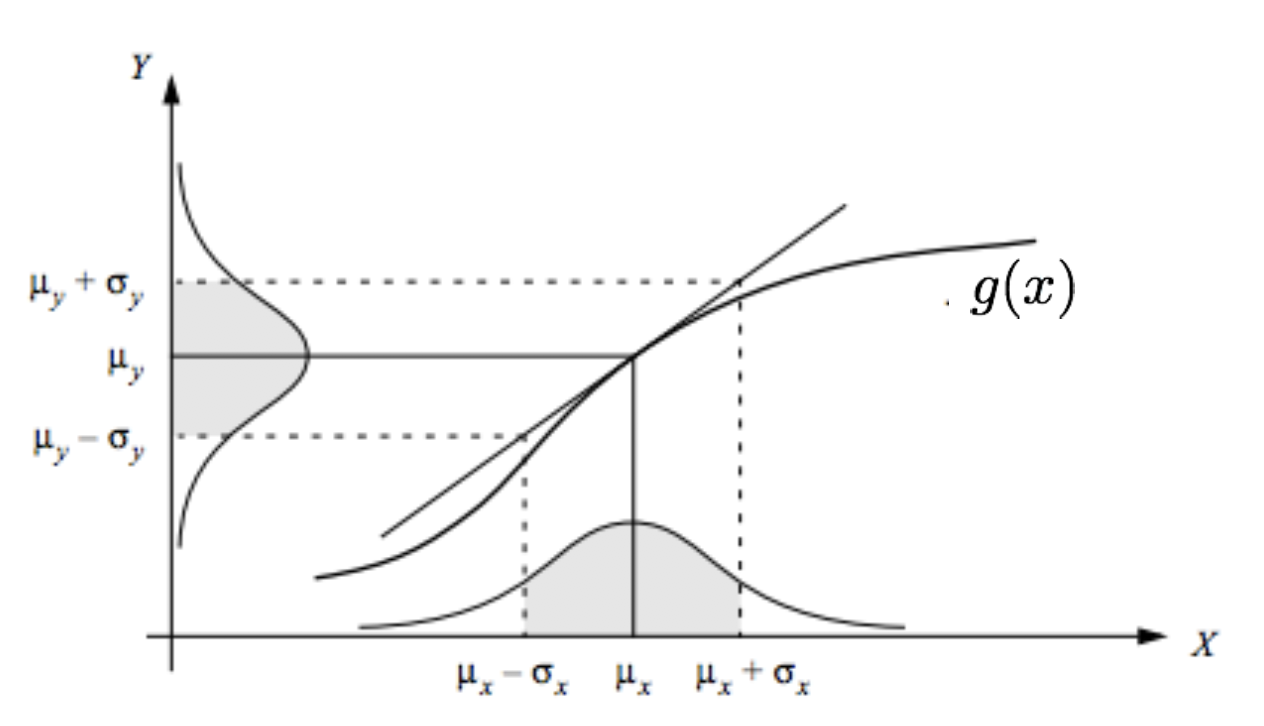
\includegraphics[width=0.6\textwidth]{ErrorPropagation_1D}
    \captionof{figure}{Variance in output vs variance in input \cite{SNS}}
    \label{fig:errorprop}
\end{center}

Performing a first order Taylor series expansion at the point $X = \mu_X$ gives
$$Y \approx g(\mu_{X}) + \left(\frac{\partial g}{\partial X}\bigg\rvert_{X=\mu_X}\right) (X-\mu_X)$$
% Moments for $Y$ variable gives our \textbf{Error Propagation Law} for a SISO system.
with mean
$$\mu_Y = g(\mu_X)$$
and variance
$$\sigma_Y^2 = \left(\frac{\partial g}{\partial X}\bigg\rvert_{X=\mu_X}\right)^2 \sigma_X^2.$$

For a more general higher-dimensional case, without delving into its complex mathematical derivation, the error propagation law can be given by 
$$\mu_{Y_j} = g_j(\mu_{X_1}, \dots, \mu_{X_n}),$$
$$C_Y = G_X C_X G_X^T$$

where $G_X, C_X, C_Y$ are the Jacobian matrix, the covariance matrix for $X$ and the covariance matrix for $Y$ given by 
\begin{center}
	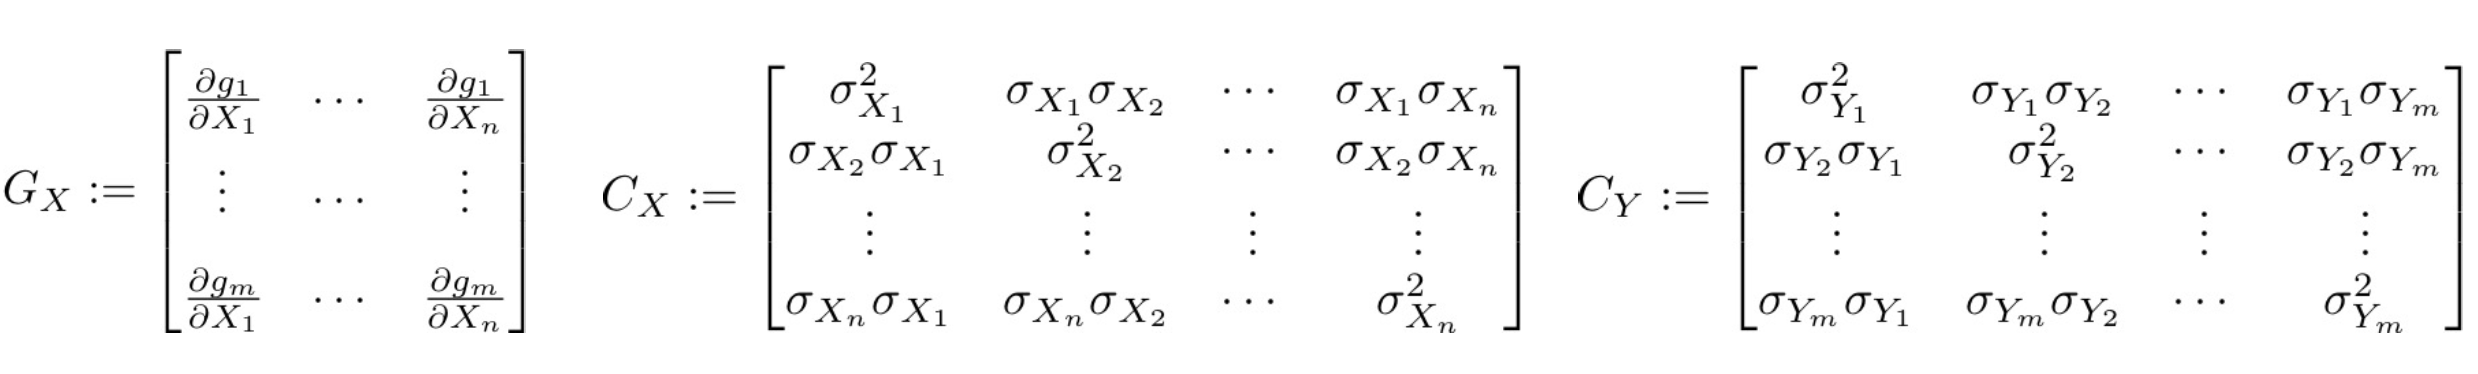
\includegraphics[width=1\textwidth]{errorpropagation_general}
\end{center}
respectively \cite{SNS}. 


\section{Geometric feature extraction}
Extracting geometric primitives (lines, circles, corners, etc) from data is extremely important for various reasons, like autonomous navigation and localization, to name a few. In this section, we focus on various methods and techniques of line extraction from range data. Since other geometric feature extraction tasks are conceptually analogous to line extraction, discussing line extraction will be sufficient for a conceptual discussion of the approach. 

The task of line extraction is achieved by \textbf{segmentation}, and then \textbf{fitting} given the association of points to a line. 

\subsection{Fitting}
The goal is to fit a line to a set of sensor measurements. For this, it is useful to work in polar coordinates as it accords importance to the reference frame of the sensor.

\begin{center}
	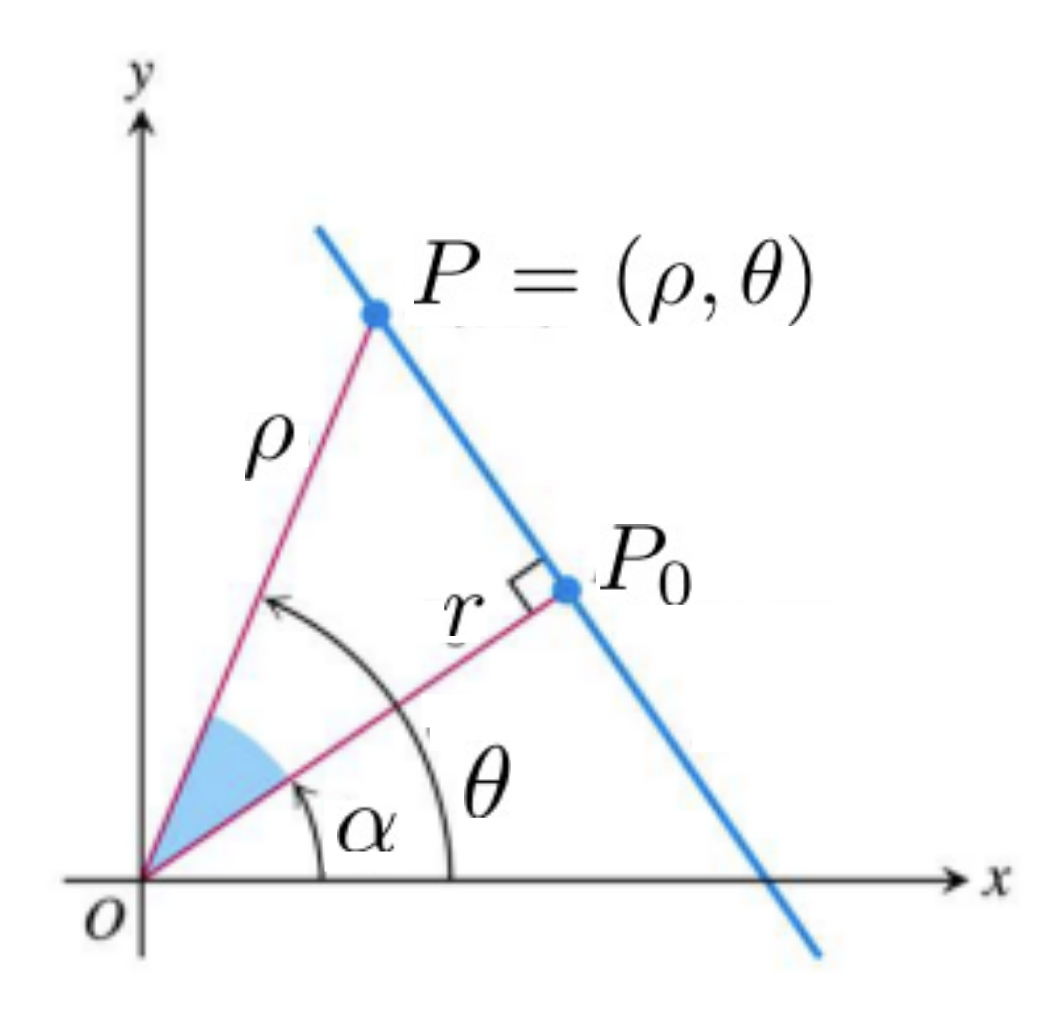
\includegraphics[width=0.5\textwidth]{PolarCoordinates}
    \captionof{figure}{Representation of line in polar coordinates}
\end{center}

\textbf{Equation of a line in polar coordinates} 

The cartesian mapping of a point in the polar coordinates is given by
$$x = \rho \cos \theta, \hspace{2mm} y = \rho \sin \theta.$$

Let $P = (\rho, \theta)$ be an arbitrary point on the line. Since $P, P_0, O$ determine a right triangle, we have
$$\rho \cos(\theta - \alpha) = r$$
or 
$$x \cos \alpha + y \sin \alpha = r$$
where $(r,\alpha)$ are the parameters of the line. 

However, there is measurement error, and the equation of line is only approximately satisfied. We can write 
$$\rho_i \cos(\theta_i - \alpha) = r + d_i$$
where $(\rho_i, \theta_i)$ is a measurement point represented in polar coordinates and $d_i$ is the corresponding error term. 

Assuming that we have $n$ ranging measurement points represented in polar coordinates as $(\rho_i, \theta_i)$, let's first consider the case when all measurements are equally uncertain. The problem then reduces to finding the line parameters $r,\alpha$ that minimizes the squared error
$$S(r,\alpha) := \sum_{i=1}^n d_i^2 = \sum_{i=1}^n(\rho_i \cos(\theta_i - \alpha) - r)^2.$$

Assuming that the $n$ ranging measurements are independent, the solution is given by the equations
$$r^* = \frac{1}{n}\sum_i^n \rho_i\cos(\theta_i - \alpha) := g_1$$ and
$$\alpha^* = \frac{1}{2} \arctan\left(\frac{\sum_i^n \rho_i^2\sin(2\theta_i) - \frac{2}{n}\sum_i^n\sum_j^n \rho_i \rho_j \cos\theta_i \sin \theta_j}{\sum_i^n \rho_i^2\cos(2\theta_i) - \frac{1}{n}\sum_i^n\sum_j^n \rho_i \rho_j \cos(\theta_i + \theta_j)}\right) + \frac{\pi}{2} := g_2.$$

Let's also consider a case where each measurement has its own unique uncertainty such that each measurement has a weight $w_i$ associated with it. In such a case, we minimize
$$S(r,\alpha) := \sum_{i=1}^n w_id_i^2 = \sum_{i=1}^n w_i(\rho_i \cos(\theta_i - \alpha) - r)^2$$
and the solution becomes \cite{SNS}
$$r^* = \frac{\sum_i^n w_i \rho_i\cos(\theta_i - \alpha)}{\sum_i w_i} := g_1$$ and
$$\alpha^* = \frac{1}{2} \arctan\left(\frac{\sum_i^n w_i \rho_i^2\sin(2\theta_i) - \frac{2}{\sum_i w_i}\sum_i^n\sum_j^n w_i w_j\rho_i \rho_j \cos\theta_i \sin \theta_j}{\sum_i^n w_i \rho_i^2\cos(2\theta_i) - \frac{1}{\sum_i w_i}\sum_i^n\sum_j^n w_i w_j \rho_i \rho_j \cos(\theta_i + \theta_j)}\right) + \frac{\pi}{2} := g_2.$$

\subsection{Segmentation}
There are several algorithms that help in the task of segmentation. Three such popular algorithms are discussed below.
\subsubsection{Split-and-merge algorithm}
It is the most popular line extraction algorithm, arguably the fastest but not as robust to outliers as other algorithms. Algorithm 1 below gives a high level understanding of its working.

\begin{center}
	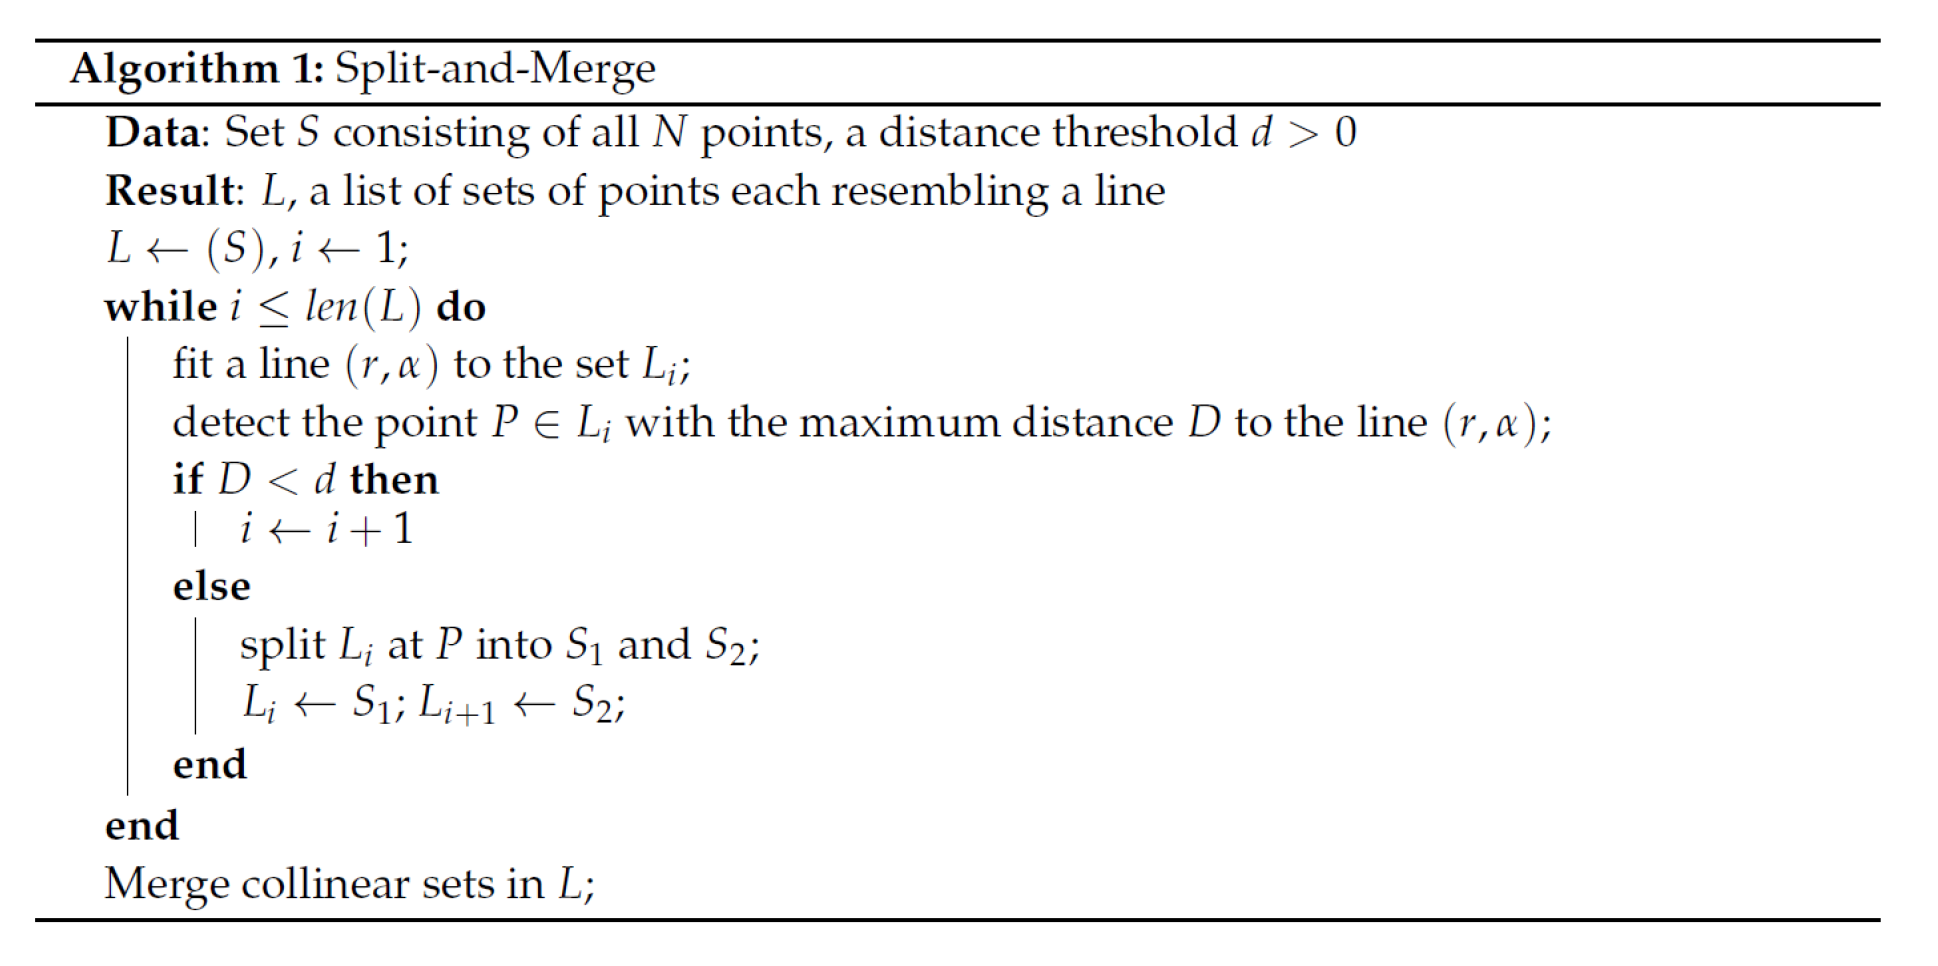
\includegraphics[width=1\textwidth]{splitandmerge}
\end{center}

There is another popular variant of split-and-merge algorithm, the Iterative-end-point-fit variant, where the primary line is constructed by simply connecting the first and the last points and then the maximum distance of the data points are compared against the distance threshold.

\begin{center}
	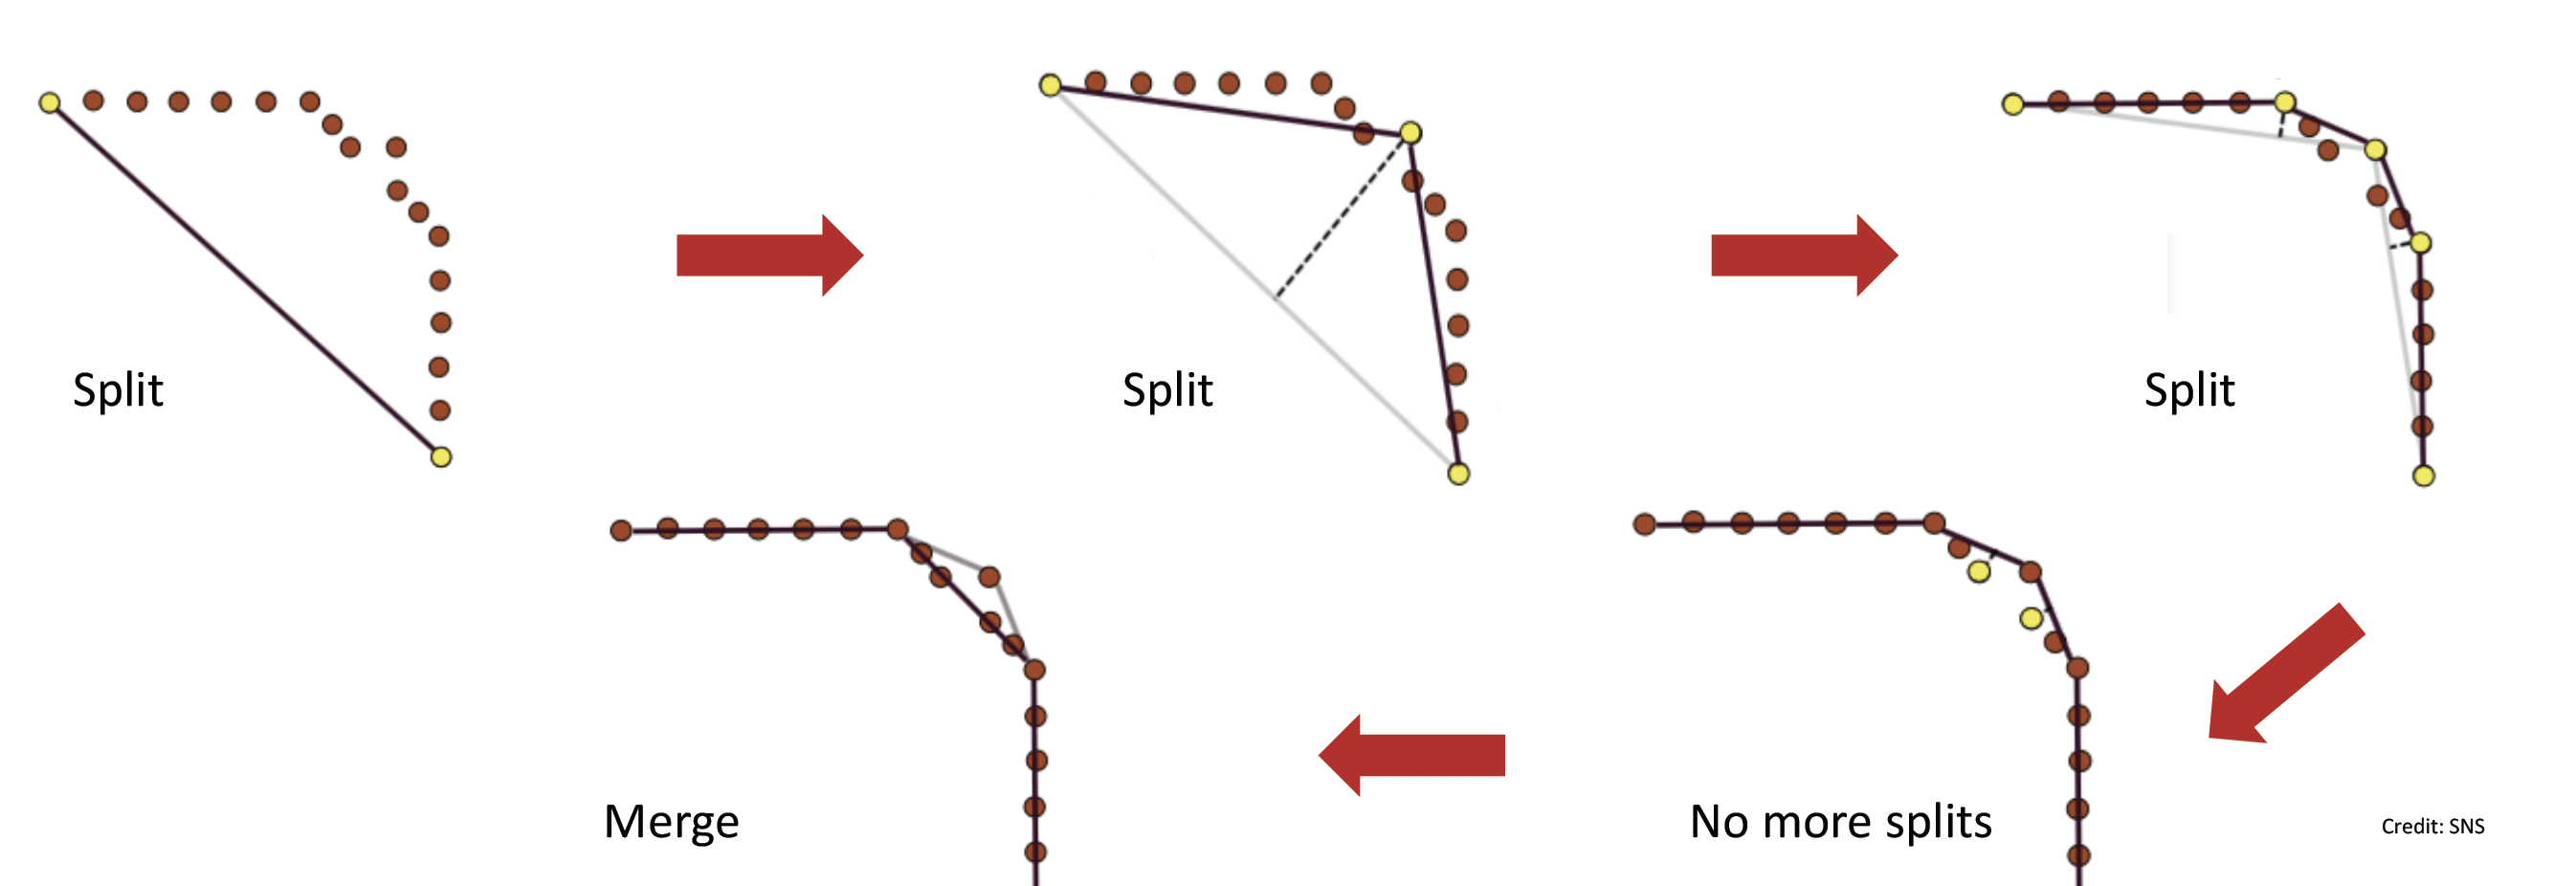
\includegraphics[width=1\textwidth]{iterativesplit}
	\captionof{figure}{Iterative-end-point-fit variant of split-and-merge algorithm \cite{SNS}}
\end{center}

\subsubsection{RANSAC (Random Sample Consensus)}
The RANSAC algorithm has wide reaching applications outside of just line segmentation. It can be used generally to find parameters of a model using a dataset with outliers. Here we will just use it for line segmentation.

RANSAC is an iterative and non-deterministic algorithm. The probability of finding a set free of outliers increases as the number of iterations increases. An overview of the algorithm as applied to line segmentation is as follows:
\begin{center}
	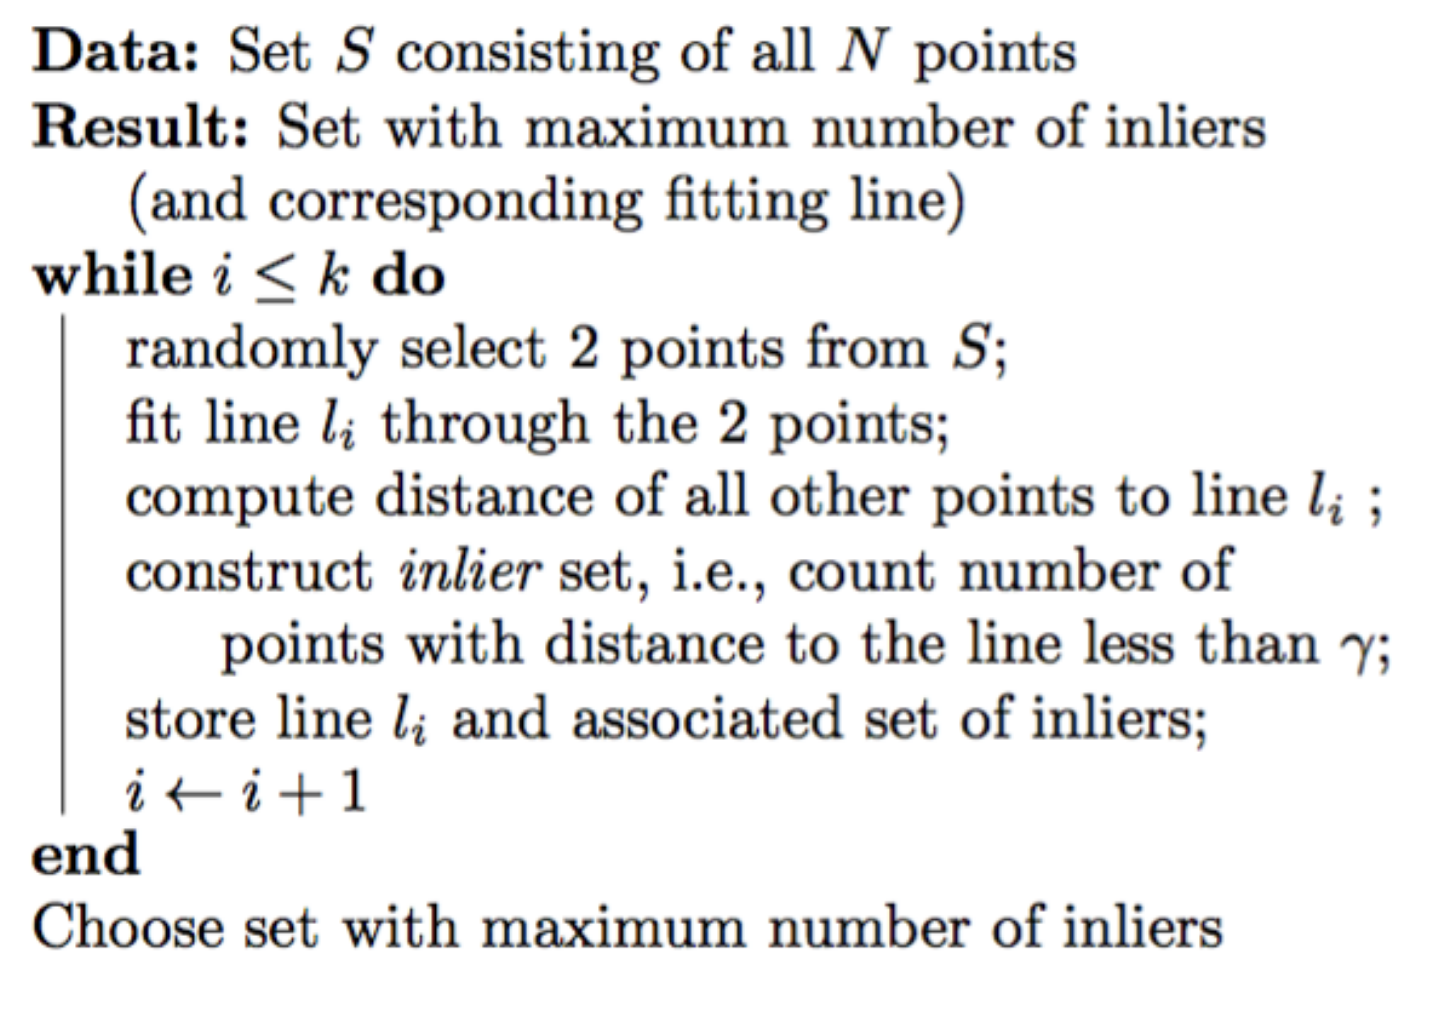
\includegraphics[width=0.5\textwidth]{RANSACOverview}
	%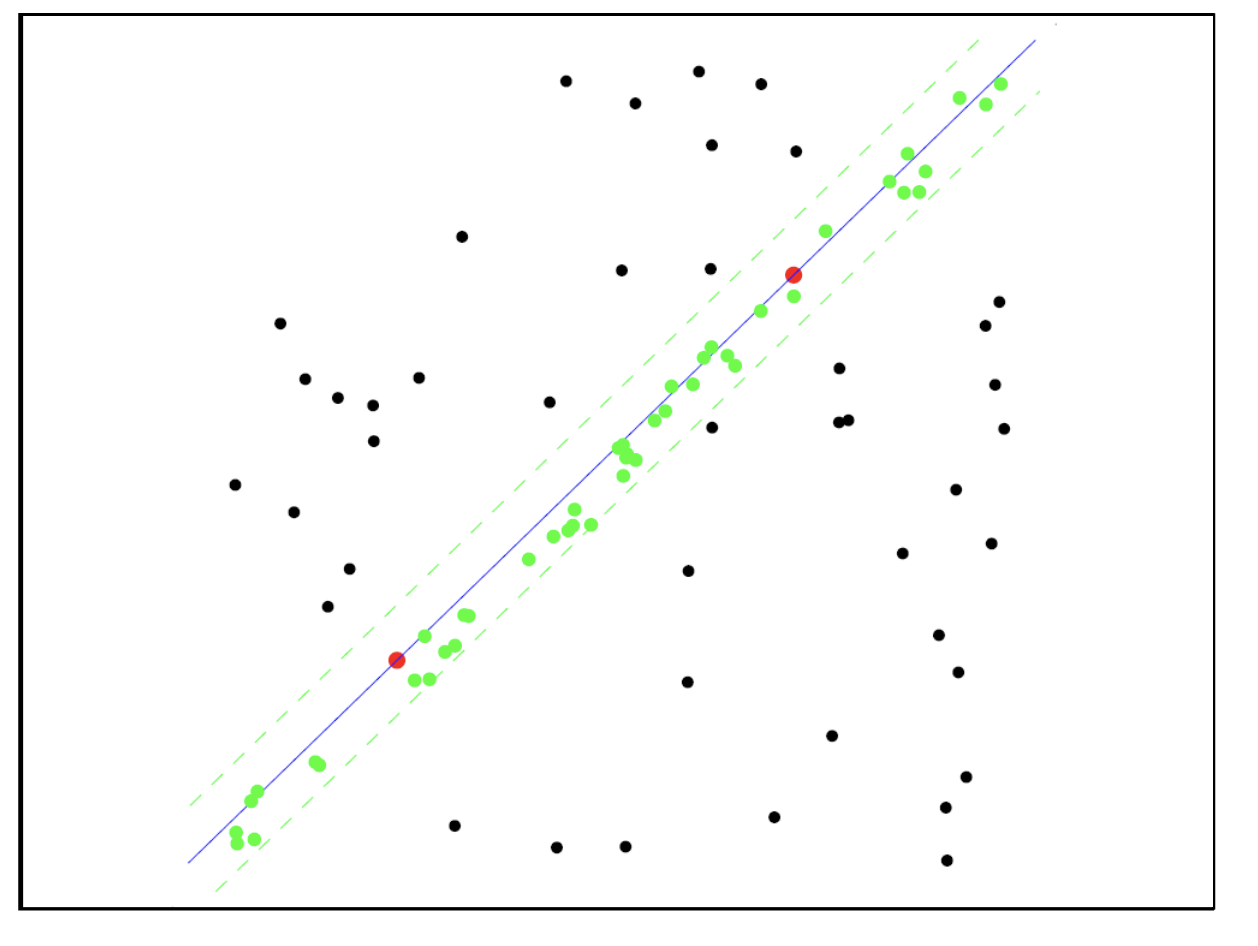
\includegraphics[width=0.5\textwidth]{RANSACEx}
\end{center}

However, this would imply that we would need to iterate through all possibilities of pairs of points in the set. If $|S| = N$, then the number of iterations needed is
$\frac{N(N-1)}{2}.$

This is too many iterations, but if we know roughly how many inliers are in the set, we can find a sufficient number of iterations. Let $w$ be the percentage of inliers in the dataset, i.e.,
$$w = \frac{\text{number of inliers}}{N},$$
and let $p$ be the desired probability of finding a set of points free of outliers (typically, we set $p=0.99$). 

We assume that 2 points chosen for line estimation are selected independently and so we have 
$$P(\text{both points selected are inliers}) = w^2.$$

Then, the minimum number of iterations $\bar{k}$ to find an outlier-free set with probability at least $p$ satisfies the equation  
$$ 1-p = (1-w^2)^{\bar{k}}.$$
Rearranging gives $$\bar{k} = \frac{\ln(1-p)}{1-w^2}.$$
Thus, if we know $w$ at least approximately, after $\bar{k}$ iterations RANSAC will find a set free of outliers with probability $p$. Of note it that $\bar{k}$ only depends on $p$ and $w$, not $N$. There are more advanced versions of RANSAC which estimate $w$ adaptively.

\subsubsection{Hough transform}
The next method is Hough transform. The key idea of this method is that each point votes for a set of plausible line parameters. 

A line has two parameters: $(m,b)$. Given a point $(x_i,y_i)$, the lines that could pass through this point are all $(m,b)$ satisfying $y_i=mx_i+b$ or $b=-mx_i+y+i$.

Thus, a point in image space $(x,y)$ maps to a line in Hough space $(m,b)$.

\begin{center}
	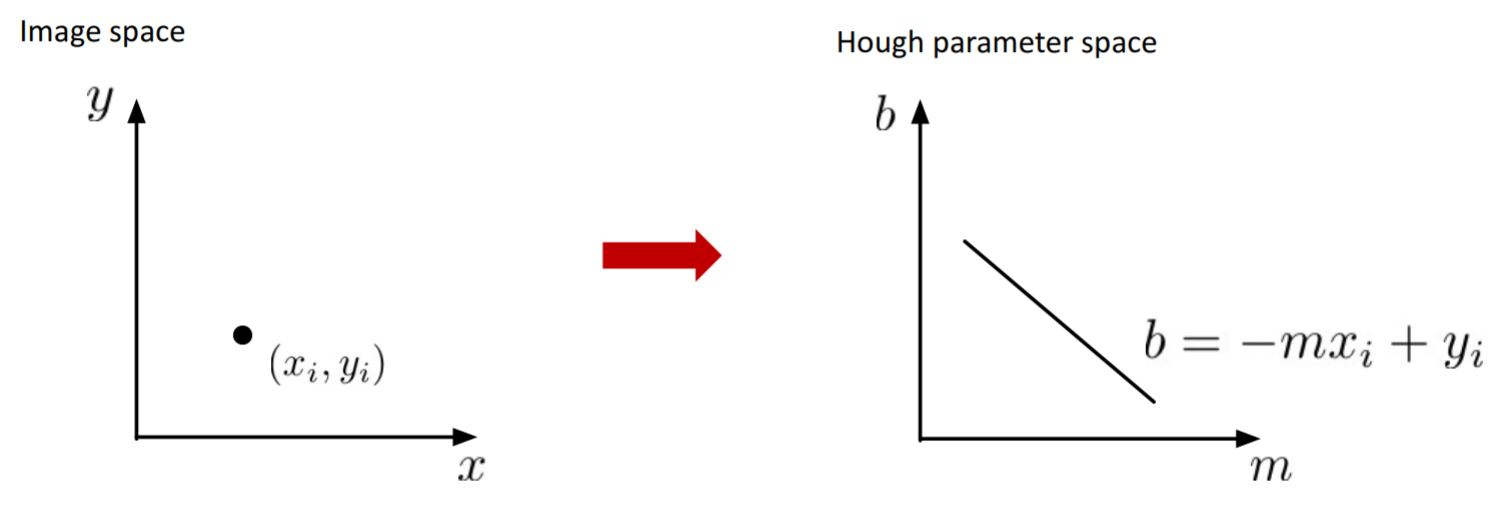
\includegraphics[width=0.75\textwidth]{hough1}
\end{center}

Two points on the same line in image space will yield two intersecting lines in Hough space.

\begin{center}
	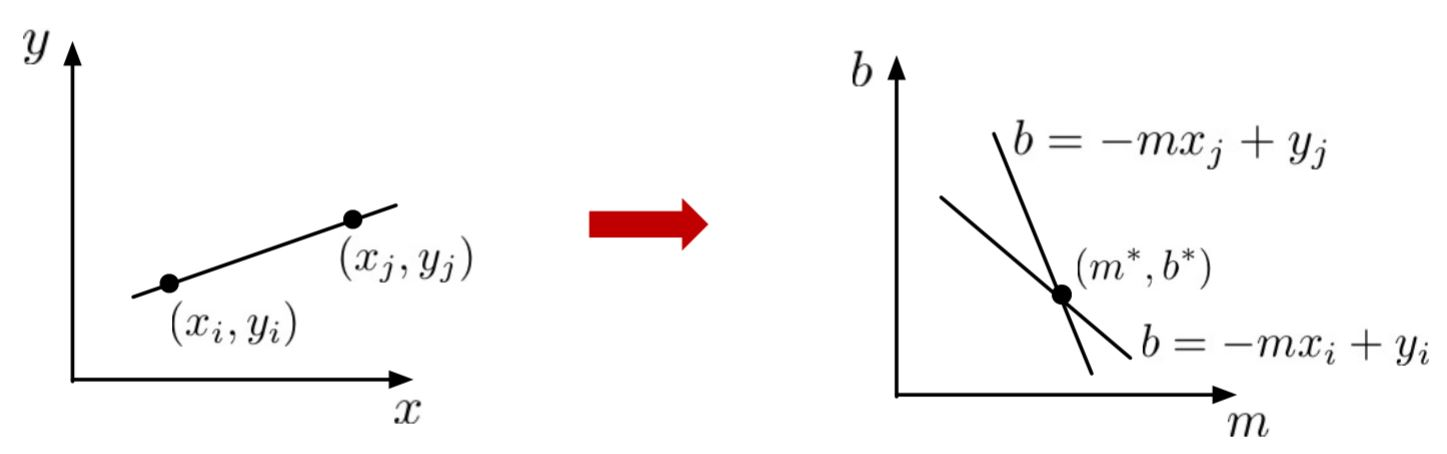
\includegraphics[width=0.75\textwidth]{hough2}
\end{center}

This concept can be applied to point segmentation. If all the points lie exactly on the same line in image space, there there will be exactly one intersection for all the lines in Hough space. Of course, this will not be true given the realities of line fitting, so instead the "center" of the many intersections will have to be estimated. One technique is to discretize the Hough space. We can perform Hough transform using the following procedure:

\begin{enumerate}
\item Initialize an accumulator array $H(m,b)$ to zero
\item For each point $(x_i, y_i)$, increment all cells that satisfy $b = -x_i m + y_i$
\item Local maxima in array $H(m,b)$ correspond to lines 
\end{enumerate}

\begin{center}
	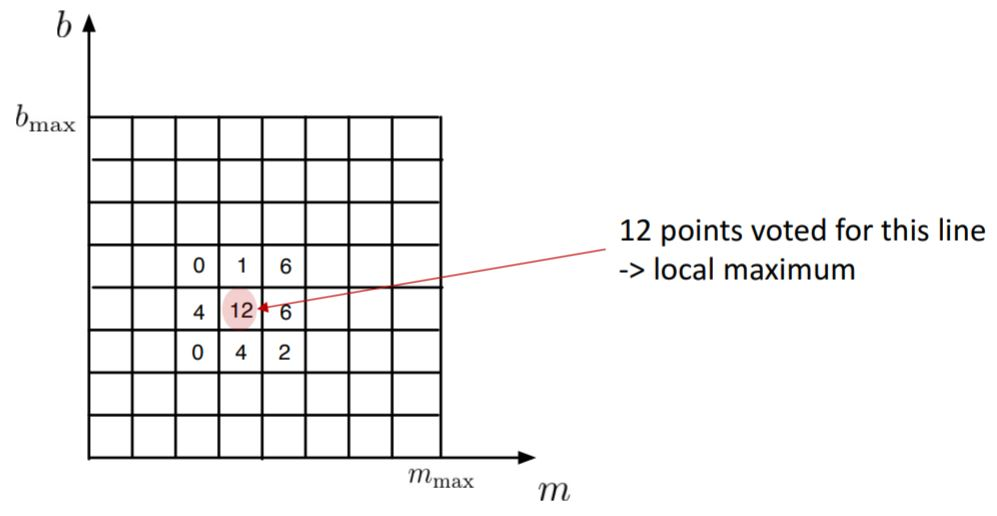
\includegraphics[width=0.6\textwidth]{hough3}
\end{center}

When performing discretization, there is an inherent tradeoff between range and resolution. This is problematic in the Hough space, since the slope $m$ can range from $-\infty$ to $\infty$. 

The solution is to transform Cartesian coordinates to polar coordinates, as covered in Section 8.3. The Hough space in polar coordinates now depends on $\alpha$ and $r$ and avoids problems associated with infinity. Instead of a line in Cartesian Hough space, we are now presented with a sinusoidal curve in polar Hough space.

\begin{center}
	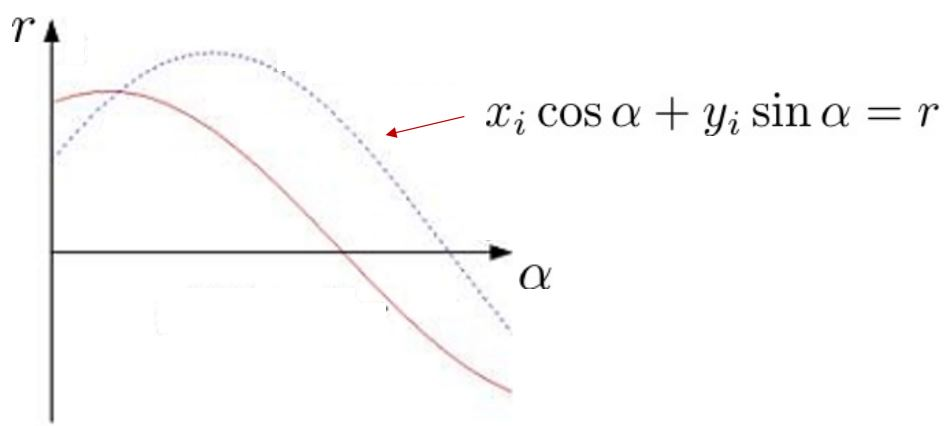
\includegraphics[width=0.5\textwidth]{hough4}
\end{center}

Below is an example featuring points that lie exactly on two lines. In Hough space two intersection points are clearly identified. These intersection points correspond with the parameters associated with the two red lines that fit the data exactly.

\begin{center}
	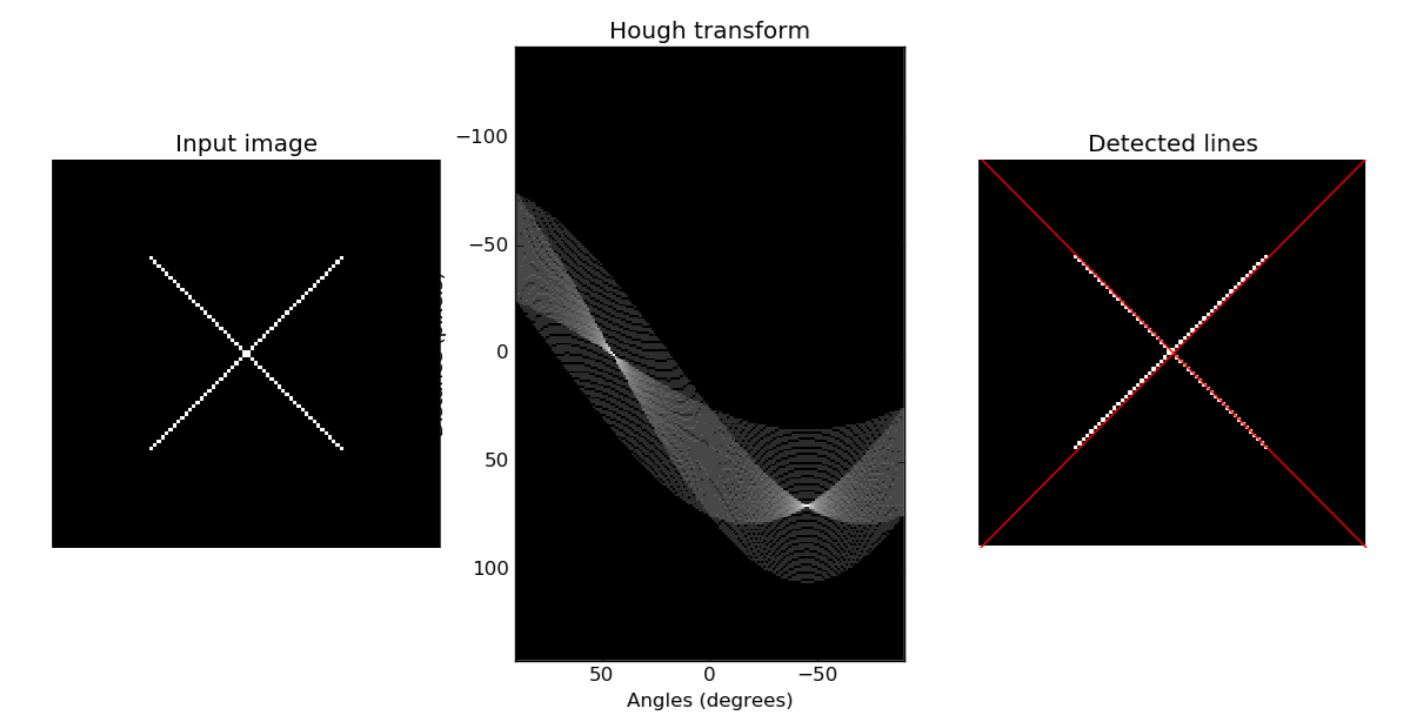
\includegraphics[width=0.6\textwidth]{hough5}
\end{center}

Given some noise, however, the intersection becomes less clear and some estimation is required.

\begin{center}
	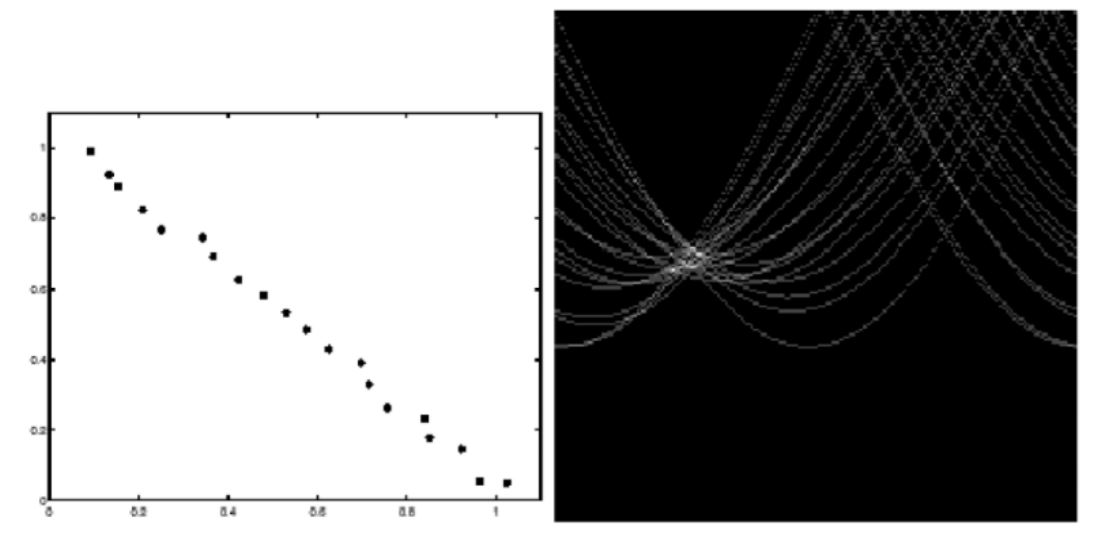
\includegraphics[width=0.5\textwidth]{hough6}
\end{center}

\subsubsection{Comparison of techniques}
RANSAC is the most general of the three algorithms. It can extract lines, curves, circles, and other geometric features. If the data has a lot of noise, this is the algorithm of choice. However, it suffers from the fact that it is a probabilistic algorithm.

Split and Merge can be intricate to implement. Its output depends heavily on parameter tuning and can take time to get right. However, it is the most computationally efficient method of the three.

Hough Transform is an elegant solution and can be seen as the middle ground of the above two techniques.

\section{Object recognition and scene understanding}
Key idea: Capture an object as a set of descriptors and compare against a dictionary to identify the object. 

We will briefly examine a technique known as Bag of Words. From an image of a duck, we might extract features such as beak, eyes, and feet. We then compare against a dictionary to check what images we have seen in th past that also contain a beak, eyes, and feet. We are given probabilities associated with past images and we select the image with the highest probability (probably a duck, probably not a raccoon).

\begin{center}
	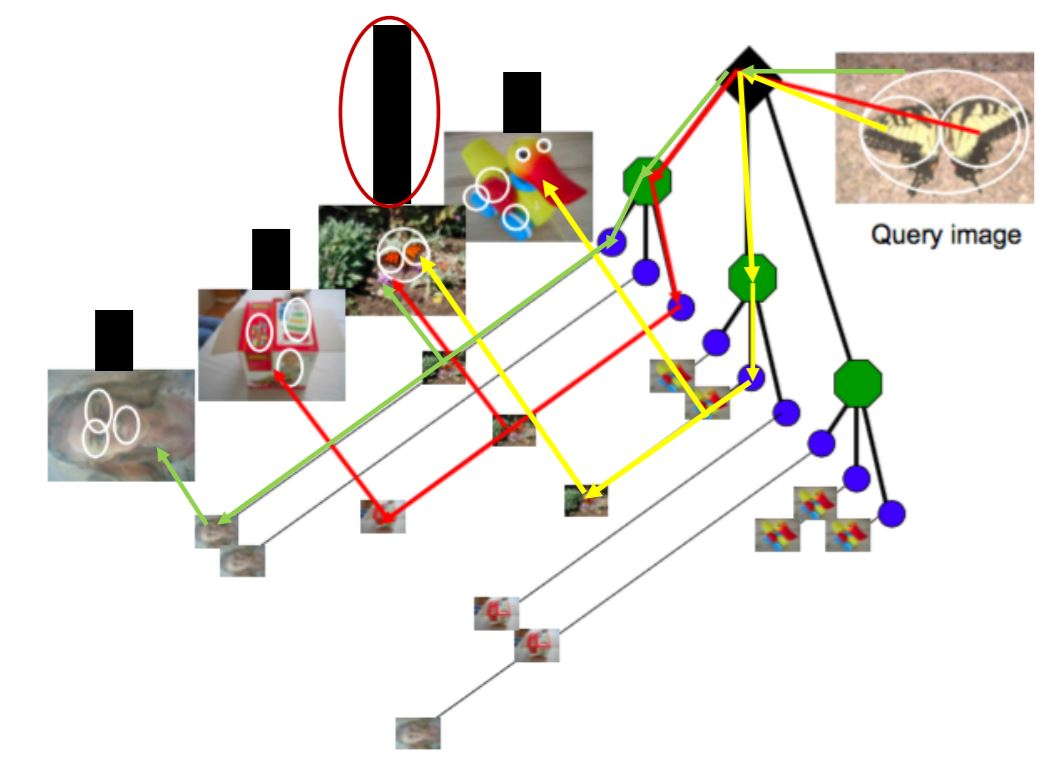
\includegraphics[width=0.6\textwidth]{bag_of_words}
\end{center}

However, these parameters are carefully engineered descriptors (features), which makes this technique rather error prone. Fortunately, machine learning offers a more automated and accurate approach.

\section{Machine Learning and Modern Visual Recognition Techniques}

Before we learn Convolutional Neural Networks (CNNs), Deep Neural Networks, or even Neural Networks, we must first understand the task that machine learning attempts to achieve. The goal of machine learning is to infer unknowns from knowns.

Machine learning can be divided into two sub-categories: (1) supervised learning, and (2) unsupervised learning.

\begin{itemize}
\item In supervised learning, we wish to choose a function $f(x) = y$ given labeled data $(x^1, y^1), \dots, (x^n, y^n)$, where $x_i =$ data point and $y_i =$ class/value.

\item In unsupervised learning, we wish to find patterns in the data $(x^1, x^2, \dots, x^n)$, which do not come with labels $y_i$, as was the case with supervised learning.
\end{itemize}

\subsection{Supervised learning}

Supervised learning algorithms can achieve two tasks: regression and classification. In regression, chosen functions mapping data to discrete-values. In classification, functions classify data into distinct categories as seen in Figure \ref{fig:supervised_learning}

\begin{figure}[!ht]%
    \centering
    \subfloat[Regression]{{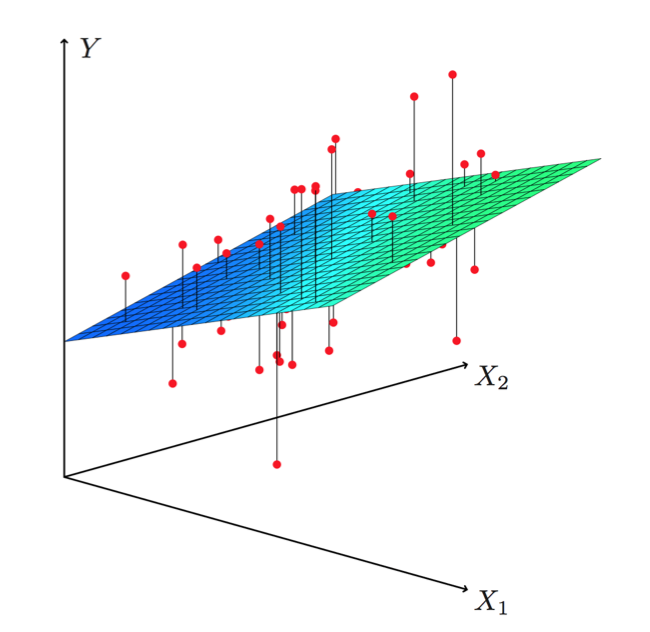
\includegraphics[width=4cm]{regression} }}%
    \qquad
    \subfloat[Classification]{{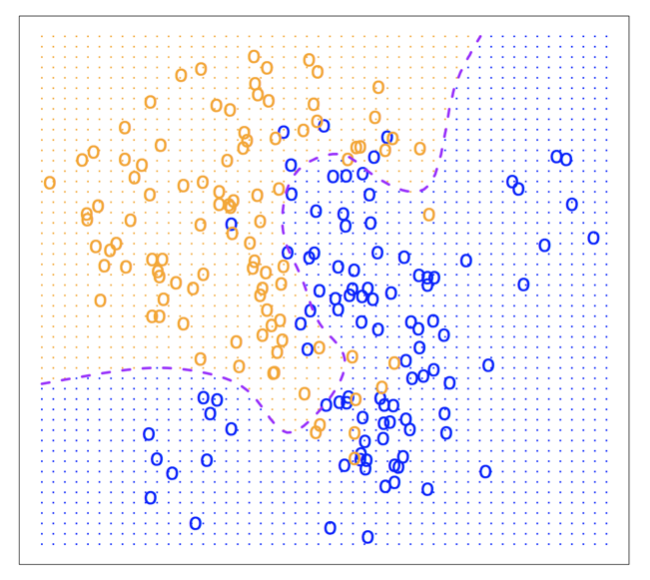
\includegraphics[width=4cm]{classification} }}%
    \caption{Supervised Learning}%
    \label{fig:supervised_learning}%
\end{figure}

\subsection{Loss Functions}

In order to select the best function $f(x) \approx y$, we must define a loss metric to be minimized.

For regression we can use the $\ell^2$ or $\ell^1$ loss. The $\ell^2$ loss is defined as:
$$\ell^2 \ Loss: \ \sum_{i} |f(x^i) - y^i|^2$$
This loss function penalizes predicted points $f(x^i)$ that are farther from true labels $y^i$ much more than those that are closer.

The $\ell^1$ loss is defined as: 
$$ \ell^1 \ Loss: \ \sum_{i} |f(x^i) - y^i|$$
This loss function penalizes predicted points $f(x^i)$ proportional to how far away they are from true labels $y^i$. Choosing the proper loss function is application and goal dependent. 

For classification, we can use a $0-1$ loss, or the cross entropy loss. The $0-1$ loss is defined as:
$$0-1 \ Loss: \ \sum_{i} \textbf{1} \{f(x^i) \neq y^i \}$$

This metric simply treats the number of times the function incorrectly classified a data point as the loss.

The cross entropy loss is defined as:
$$Cross\ Entropy\ Loss: \ -\sum_{i} (y^i)^T \log{f(x^i)}$$

\subsection{Learning Models}

\begin{figure}[!ht]%
    \centering
    \subfloat[Linear Regression]{{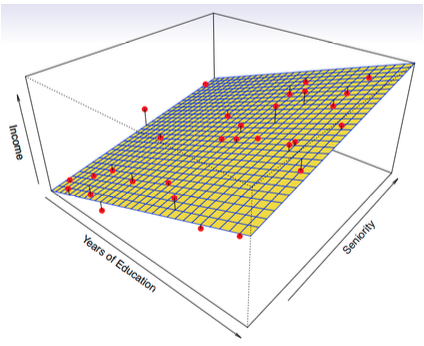
\includegraphics[width=4cm]{linear_regression} }}%
    \qquad
    \subfloat[Linear Classifier]{{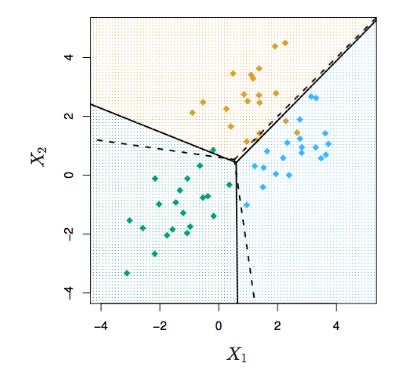
\includegraphics[width=4cm]{linear_classifier} }}%
    \caption{Examples of Parametric Models}%
    \label{fig:parametric_models}%
    \subfloat[Spline Fitting]{{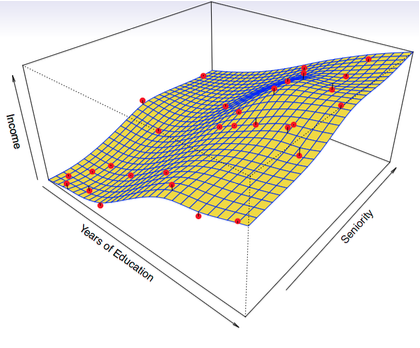
\includegraphics[width=4cm]{spline_fitting} }}%
    \qquad
    \subfloat[k-Nearest Neighbors]{{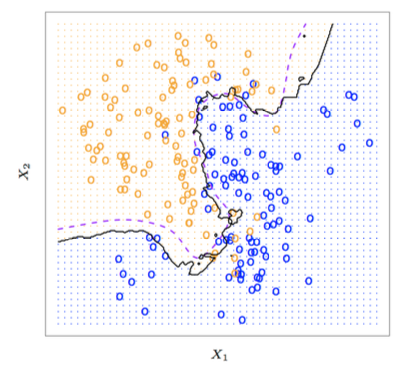
\includegraphics[width=4cm]{knn} }}%
    \caption{Examples of Nonparametric Models}%
    \label{fig:nonparametric_models}%
\end{figure}

There are two approaches to learning functions or models for classification and regression tasks. Parametric models, such as linear regression or linear classifiers, are functions represented by parameters (see Figure \ref{fig:parametric_models}).

Non-parametric models do not depend on parameters. For example, non-parametric spline fitting involves building up piecewise models to fit the data. k-Nearest Neighbors classifies samples based on the class most common amongst its k nearest neighbors. This algorithm approximates the test set value using the values from its neighbors in the training set. k nearest neighbor algorithm is mostly used in image compression. See Figure \ref{fig:nonparametric_models}. Other non parametric algorithms include support vector machines and the EM algorithm. 


\subsection{Machine Learning as Optimization}

For parametric models, how do we select the best parameters to fit the training data? Analytical approaches to solving this problem include least squares. For large datasets, however, this may pose computational challenges. Other popular approaches include numerical methods, such as gradient descent.

Full gradient descent may be computationally inefficient, as each iteration requires a computation over the entire batch of training data. Instead, we can use stochastic gradient descent (Figure \ref{fig:sgd}) or batch gradient descent, which compute gradients over small portions of the training data with each iteration. 

\begin{figure}[!ht]%
    \centering
    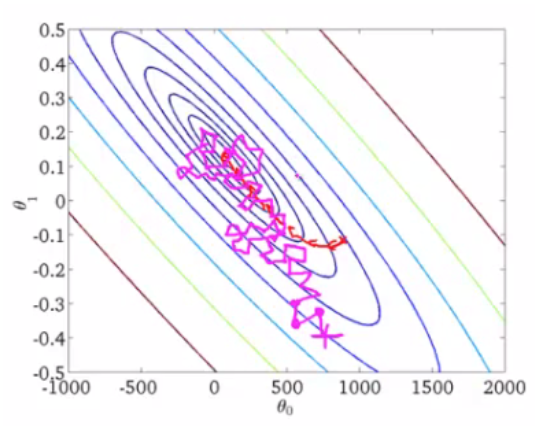
\includegraphics[width=5cm]{sgd}
    \caption{Stochastic Gradient Descent}
    \label{fig:sgd}%
\end{figure}

\subsection{Machine Learning as Optimization}

The overarching goal of machine learning is to perform well on unseen data. As such, we must avoid over-fitting on the training data to ensure that model performance generalizes to test data. We can perform regularization by adding additional terms to the loss function to penalize "model complexity". 

\begin{itemize}
\item $\ell^2$ regularization: $\|A\|_2$ often corresponds to a Gaussian prior on parameters $A$. 

\item $\ell^1$ regularization: $\|A\|_1$ often encourages sparsity in $A$ (easier to interpret/explain).
\end{itemize}

Regularization can also be performed by tuning hyperparameters relevant to the learning model. For example, with k-Nearest neighbors, larger values for $k$ result in greater regularization as seen in (a) of Figure \ref{fig:hyper_parameters}.

For kNN, plotting the training error and test errors with respect to $\frac{1}{k}$ allows us to determine the optimal hyperparameter value. As seen in (b) of Figure \ref{fig:hyper_parameters}, larger $k$ achieves improved performance, but beyond $\frac{1}{k} = 0.1$, the test error increases due to overfitting.

\begin{figure}[!ht]%
    \centering
    \subfloat[k-Nearest Neighbors]{{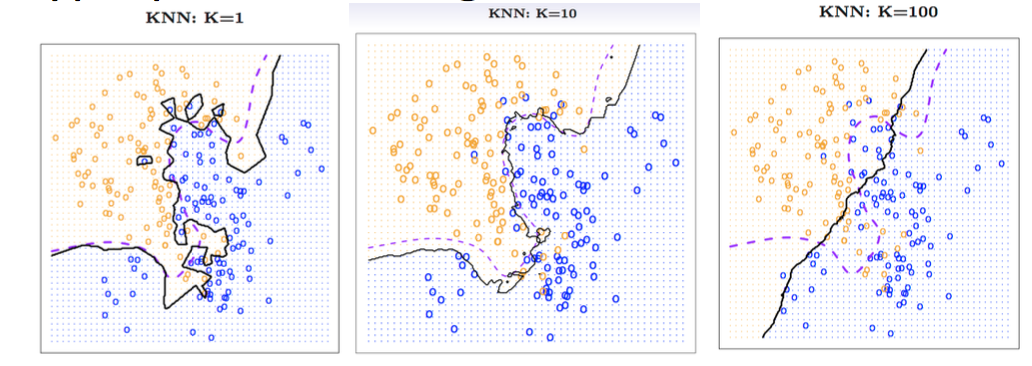
\includegraphics[width=10.5cm]{hyper_parameters} }}%
    \qquad
    \subfloat[Determining Optimal Value for k]{{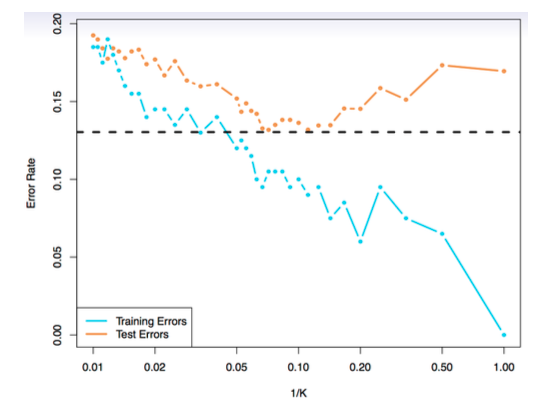
\includegraphics[width=5cm]{bias_vs_var} }}%
    \caption{Hyperparameter Regularization}%
    \label{fig:hyper_parameters}%
\end{figure}


\subsection{Linear classifiers}

A linear classifier can be defined by the following function:
$$f(x, W) = W x + b $$
where $W$ are weights/parameters, and $b$ is a bias term.

For example let's say we are trying to classify RGB images of size 32x32 into one of 3 classes: cats, dogs, or ships (see Figure \ref{fig:cat_classifier}). Multiplying 32x32 pixels by 3 RGB colors, input $x$ is a vector of size $(3072,\ 1)$, $W$ is a matrix of size $(10,\ 3072)$, $b$ is a vector of size $(3,\ 1)$, and output $f(x, W)$ is also a vector of size $(3,\ 1)$, with each element assigning a score to each class.

\begin{figure}[!ht]%
    \centering
    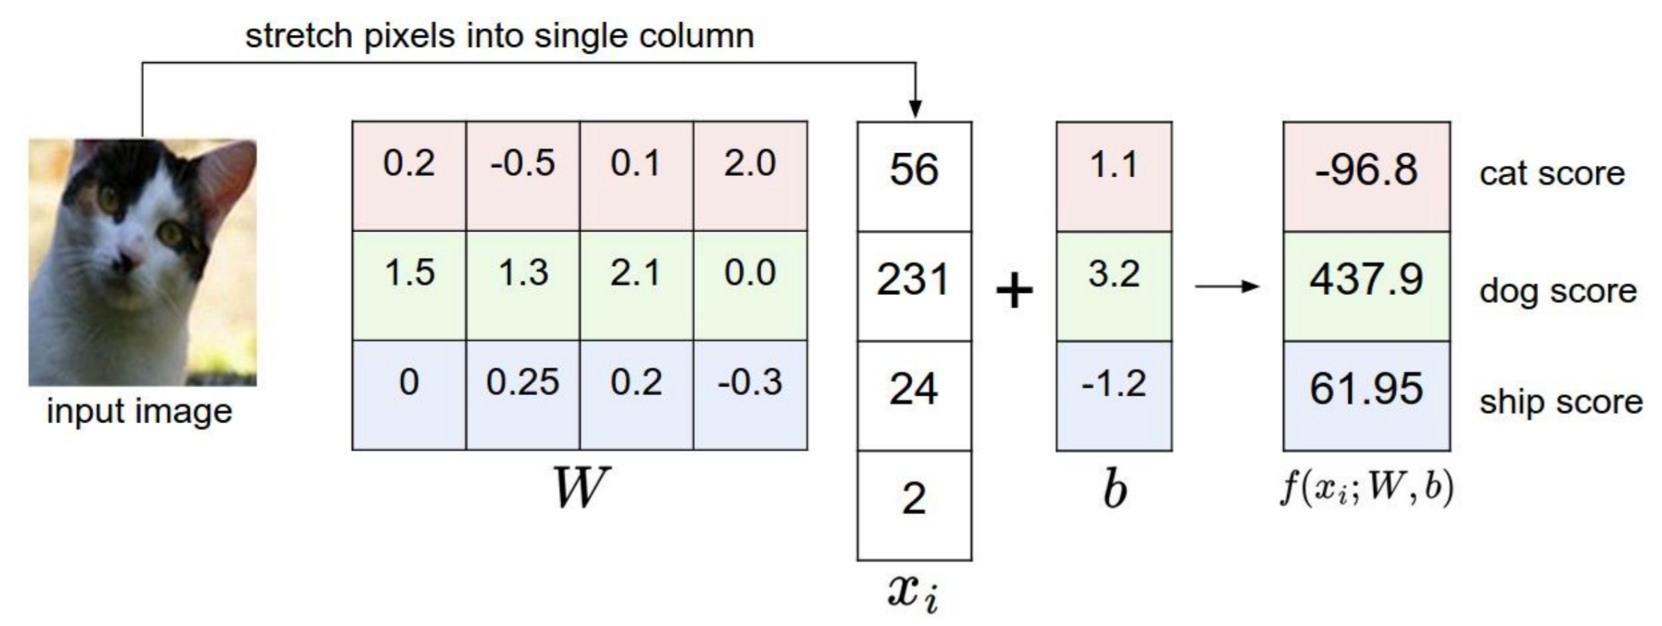
\includegraphics[width=14cm]{cat_classifier}
    \caption{Example Linear Classifier}
    \label{fig:cat_classifier}%
\end{figure}

Note that each row of matrix $W$ performs a dot product operation with input $x$, which combined with bias $b$, produces a score corresponding to a particular class. We can interpret each row of matrix $W$ as a "template" performing nearest neighbor classification. The elements of each row are ideally weighted such that pixel values that tend to be associated with a particular class will produce a higher score in the class associated with said row.

\subsection{Dot Products as a Measure of Similarity}

The concept of dot products can also give us some insight into what makes a good classifier.
The dot product is defined as:
$$w^T x = \|w\| \|x\| \cos \theta$$
Cosine similarity is described by the following:
$$\cos(\theta) = \frac{w^Tx}{\| w \| \|x\|} $$

We can interpret the linear classifier as performing projections that determine "how much" of each row of weights $w$ associated with a particular class are in input $x$. When weights $w$ and input $x$ are similar, $\cos(\theta) \approx 1$. When they are not similar, $\cos(\theta) \approx -1$.



\subsection{Generalized Linear Models}
Linear regression and classification  are special cases of a broad family of models called Generalized Linear Models. In a generalized linear model, each outcome $Y$ of the dependent variables is assumed to be generated from a particular distribution in the exponential family, a large range of probability distributions that includes the normal, binomial, Poisson and gamma distributions, among others \cite{10.2307/2344614}. 

\begin{itemize}
\item To start with, first let us define an exponential family. We say that a class of distribution is in the exponential family if it can be written in the following form:
\[p(y;\eta) = b(y) \exp(\eta^T T(y) - a(\eta)).\] 
Here, $\eta$ is the natural parameter, $T(y)$ is the sufficient statistic, and $a(\eta)$ is the log partition function. The quantity $e^{-a(\eta)}$ essentially plays the role of the normalization constant that makes the distribution sum to $1$. To give an example, let us see how a Bernoulli equation can be written as an exponential family.
\[ p(y;\phi)  = \phi^y(1-\phi)^{1-y}\]
\[p(y;\phi)  = \exp \left(\left(\log \left(\frac{\phi}{1-\phi}\right)\right)y + \log(1-\phi) \right) \]
Here, the natural parameter is $\eta = \log \left(\frac{\phi}{1-\phi}\right)$.

\item Constructing GLMs \\
Consider a classification or regression problem, where we want to estimate the value of some random variable $y$, as a function of $x$. We make certain assumptions to generate the GLM. These assumptions are: 
\begin{itemize}
\item  Given $x$ and parameters $\theta$, $y$ follows an exponential family distribution with some natural parameter $\eta$.
\item The output $h(x)$ of our learned hypothesis $h$ satisfies the equation $h(x) = E[y|x]$
\item The natural parameter $\eta$ is linearly related to the inputs $x$: $\eta = \theta^Tx$
\end{itemize} 
Thus a GLM consists of a probability distribution from the exponential family, a linear predictor $\eta = \theta^Tx$, and a link function: $E(y) = g^{-1}(\eta)$. The canonical link function provides a relation ship between the mean $\mu$ of $y|x$, and the natural parameter $\eta$.

\end{itemize} 

\subsection {Softmax Regression}
Softmax Regression is another special case of a GLM. Consider a classification problem where the variable $y$ can take $k$ values from $0$ to $k$. This is an extension to the binary classification problem we saw before for which we used logistic regression. From the general GLM model, it can be derived that the conditional probability distribution of $y$ is given as follows: \\

\[p(y=i;x,\theta) = \frac{e^{\theta_i^T(x)}}{\sum_{j=1}^k\theta_j^T(x)}\]
Thus Softmax regression is a generalization of logistic regression. Our model will output the following hypothesis function:
\[h_{\theta}(x) = \begin{bmatrix}\frac{e^{\theta_1^T(x)}}{\sum_{j=1}^k\theta_2^T(x)}\\\frac{e^{\theta_1^T(x)}}{\sum_{j=1}^k\theta_j^T(x)} \\
.\\
.\\
\frac{e^{\theta_k^T(x)}}{\sum_{j=1}^k\theta_j^T(x)} \end{bmatrix}\]

In other words, our hypothesis will output the estimated probability that $p(y = i|x; θ)$, for every value of $i = 1, . . . , k$.



\subsection{Histogram of Oriented Gradients (HOG)}
The histogram of oriented gradients is a feature descriptor used for object detection in computer vision and machine learning \cite{wikipedia_2017}.
Local object appearance and shape within an image can be described by the distribution of intensity gradients or edge directions. The image is divided into small connected regions called cells, and for the pixels within each cell, a histogram of gradient directions is compiled. The descriptor is the concatenation of these histograms. For improved accuracy, the local histograms can be contrast-normalized by calculating a measure of the intensity across a larger region of the image, called a block, and then using this value to normalize all cells within the block. This normalization results in better invariance to changes in rotation, scale, intensity, and viewpoint change.
Calculating the HOGs involves the following steps: \\

\begin{itemize}
\item \textbf{Gradient Computation:}
Computing gradient values using masks, e.g. 1-D masks for horizontal, vertical or both directions. This filters the color or intensity data of the image by using filters.

\item \textbf{Orientation binning:} 
In this step, we create cell histograms. Each pixel in the cell has a weight for the histogram found by gradient computation. The histogram channel is $0-\ang{180} $ or $0-\ang{360}$  based on if the histogram has a sign or not.

\item \textbf{Descriptor blocks:}
HOG descriptor is the concatenated vector of the components of the normalized cell histograms from all of the block regions. This accounts for changes in illumination and contrast by grouping cells into larger blocks. Each cell contributes more than once to the final descriptor since generally these blocks coincide.

\item \textbf{Block Normalization:}
We can use number of normalization methods like L2 normalization for normalizing the descriptor blocks.

\item \textbf{Object Recognition:}
We can provide HOG descriptors to machine learning algorithms like support vector machines. as features.

\end{itemize}


\subsection{Feature Extraction}
Feature extraction is a technique that reduces the amount of information required to learn from large data sets. The selected features are expected to contain the relevant information from the input data, so that the desired task can be performed by using this reduced representation instead of the complete initial data. Convoluted neural nets are great tools to extract and learn complex features with relatively few neurons. 

\bibliographystyle{alpha}
\bibliography{sample}

\end{document}